\documentclass[tikz,border=10pt]{standalone}
\usepackage{tkz-euclide} % 基于TikZ，专门用于平面几何绘图

\begin{document}

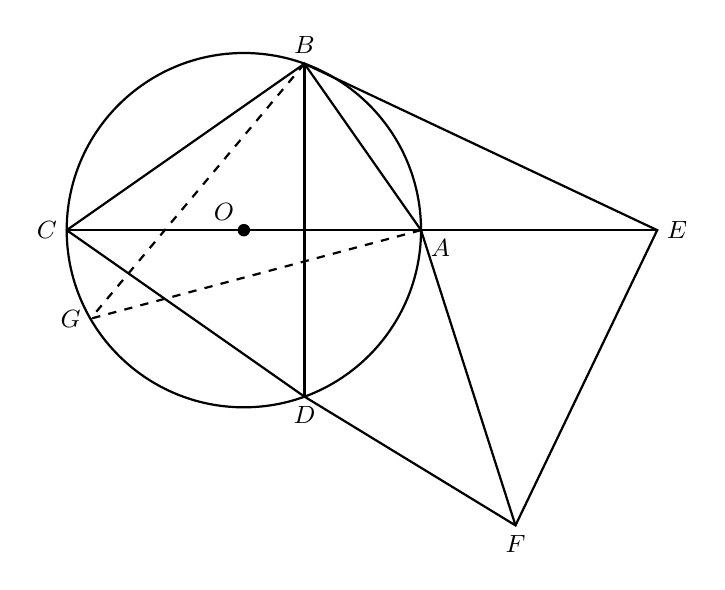
\begin{tikzpicture}[scale=1.5, font=\small]
    % 1. 定义核心点 (以O为原点，半径为2)
    \coordinate (O) at (0,0);
    \def\r{1.5} % 圆半径
    
    % 2. 定义圆上的点 (极坐标定义保证几何关系精确)
    \coordinate (C) at (180:\r);
    \coordinate (A) at (0:\r);
    \coordinate (B) at (70:\r);  % 估计B点位置
    \coordinate (D) at (-70:\r); % 估计D点位置，BD垂直AC
    \coordinate (G) at (210:\r); % 圆上的G点
    
    % 3. 定义外部延伸点
    % 寻找E点：在CA延长线上
    \coordinate (E) at (3.5, 0);
    % 寻找F点：CD延长线与EF的交点（此处根据视觉比例手动标注，或计算交点）
    \coordinate (F) at (2.3, -2.5);
    
    % 4. 绘制圆形
    \draw[thick] (O) circle (\r);
    
    % 5. 绘制实线路径 (主体轮廓)
    \draw[thick] (C) -- (B) -- (E) -- (F) -- (D) -- (C); % 外围轮廓
    \draw[thick] (C) -- (A) -- (E); % 直径及延长线
    \draw[thick] (B) -- (D);       % 弦BD
    \draw[thick] (A) -- (B);       % 弦AB
    \draw[thick] (A) -- (F);       % 连线AF
    
    % 6. 绘制虚线 (辅助线)
    \draw[dashed, thick] (B) -- (G);
    \draw[dashed, thick] (A) -- (G);
    
    % 7. 绘制点和标签
    \foreach \p/\pos in {O/above left, A/below right, B/above, C/left, D/below, E/right, F/below, G/left}
        \fill (\p) circle (0.3pt) node[\pos] {$\p$};
    
    % 特殊标注：圆心O点加重
    \fill (O) circle (1.5pt);

\end{tikzpicture}

\end{document}